\documentclass[11pt,a4paper]{article}

% ── Packages ──
\usepackage[utf8]{inputenc}
\usepackage[T1]{fontenc}
\usepackage{amsmath,amssymb,amsthm}
\usepackage{mathtools}
\usepackage{booktabs}
\usepackage{hyperref}
\usepackage{graphicx}
\usepackage[margin=1in]{geometry}
\usepackage{enumitem}
\usepackage{xcolor}
\usepackage{tcolorbox}

% ── Theorem environments ──
\newtheorem{theorem}{Theorem}[section]
\newtheorem{proposition}[theorem]{Proposition}
\newtheorem{lemma}[theorem]{Lemma}
\newtheorem{corollary}[theorem]{Corollary}
\newtheorem{conjecture}[theorem]{Conjecture}
\theoremstyle{definition}
\newtheorem{definition}[theorem]{Definition}
\newtheorem{remark}[theorem]{Remark}

% ── Note environment for research flags ──
\newtcolorbox{researchnote}{
  colback=orange!5!white,
  colframe=orange!75!black,
  fonttitle=\bfseries,
  title=Research Note,
  sharp corners,
  boxrule=0.5pt
}

% ── Shortcuts ──
\newcommand{\vv}{\mathbf{v}}
\newcommand{\kk}{\mathbf{k}}
\newcommand{\qq}{\mathbf{q}}
\newcommand{\oo}{\mathbf{o}}
\newcommand{\rr}{\mathbf{r}}
\newcommand{\bb}{\mathbf{b}}
\newcommand{\ww}{\mathbf{w}}
\newcommand{\zz}{\mathbf{z}}
\newcommand{\bmu}{\boldsymbol{\mu}}
\newcommand{\beps}{\boldsymbol{\epsilon}}
\newcommand{\Var}{\mathrm{Var}}
\newcommand{\Cov}{\mathrm{Cov}}
\newcommand{\Tr}{\mathrm{Tr}}
\newcommand{\KL}{\mathrm{KL}}
\newcommand{\MSE}{\mathrm{MSE}}
\newcommand{\Bias}{\mathrm{Bias}}
\newcommand{\softmax}{\mathrm{softmax}}
\newcommand{\diag}{\mathrm{diag}}
\DeclareMathOperator*{\argmin}{arg\,min}

% ══════════════════════════════════════════════════════════════════
\title{Sampling vs.\ Segmentation:\\
A Mathematical Framework for Attention Approximation}

\author{Gulcelik \and Shemla}
\date{March 2026 — Working Draft}

\begin{document}
\maketitle

\begin{abstract}
We formalize two computational models for approximating the attention output
$\oo^{*}=\sum_{i}w_{i}\vv_{i}$: \emph{sampling} (draw $B$ indices, correct
via importance weighting) and \emph{segmentation} (partition keys into $C$
groups, precompute representatives, sum over groups).  We derive variance
lower bounds for sampling, bias decompositions for segmentation, and a
crossover condition under which the deterministic bias of segmentation yields
lower MSE than the variance of unbiased sampling.  We then disentangle the
segmentation framework into two independent design choices---\emph{how to
partition} and \emph{how to choose representatives}---and analyze query-independent
versus query-dependent representative strategies including averaged keys,
nearest-value key selection, random Fourier features, and within-cluster
importance weighting.  Empirical
results on Llama-3-8B attention snapshots confirm that segmentation with 100
clusters achieves 35\% lower error than oracle importance sampling at the last
layer, while sampling dominates at the first layer, consistent with the
theoretical crossover framework.
Five ablation experiments validate the crossover formula (log-correlation 0.96),
identify weight distortion as the dominant bias source (84\% of error at the
first layer), and show that non-monotonicity in cluster count is a fitting
artifact resolved by $k$-means.
\end{abstract}

\tableofcontents
\newpage

% ══════════════════════════════════════════════════════════════════
\section{Problem Setup}\label{sec:setup}

We approximate the attention output
\begin{equation}\label{eq:attention}
  \oo^{*}
  = \sum_{i=1}^{N} w_i\,\vv_i,
  \qquad
  w_i = \softmax\!\Bigl(\frac{\qq^{\!\top}\kk_i}{\sqrt{d}}\Bigr)_{\!i}\,,
\end{equation}
where $\qq\in\mathbb{R}^{d}$ is the query,
$\{\kk_i\}_{i=1}^{N}\subset\mathbb{R}^{d}$ are keys,
$\{\vv_i\}_{i=1}^{N}\subset\mathbb{R}^{d}$ are values,
$w_i\ge0$, and $\sum_{i}w_i=1$.
We write $z_i = \qq^{\!\top}\kk_i/\sqrt{d}$ for the logits and
$\tilde{w}_i = e^{z_i}$ for the unnormalized weights.

We compare two computational models:

\begin{center}
\begin{tabular}{lll}
\toprule
\textbf{Model} & \textbf{Description} & \textbf{Budget}\\
\midrule
Sampling      & Draw $B$ indices, IS-corrected average & $B$ samples\\
Segmentation  & Partition into $C$ groups, sum over representatives & $C$ groups\\
\bottomrule
\end{tabular}
\end{center}

% ══════════════════════════════════════════════════════════════════
\section{Model~I: Sampling-Based Approximation}\label{sec:sampling}

\subsection{General Importance Sampling}

Draw $B$ i.i.d.\ indices $i_1,\dots,i_B$ from a proposal $q=(q_1,\dots,q_N)$
with $q_i>0$.  The IS estimator
\begin{equation}\label{eq:IS}
  \hat{\oo}_{\mathrm{IS}}
  = \frac{1}{B}\sum_{j=1}^{B}\frac{w_{i_j}}{q_{i_j}}\,\vv_{i_j}
\end{equation}
is unbiased: $\mathbb{E}[\hat{\oo}_{\mathrm{IS}}]=\oo^{*}$ for every $q$.
Its trace-variance across all $d$ dimensions is
\begin{equation}\label{eq:IS-var}
  \Tr\bigl(\Cov(\hat{\oo}_{\mathrm{IS}})\bigr)
  = \frac{1}{B}\biggl[\sum_{i=1}^{N}\frac{w_i^{2}}{q_i}\|\vv_i\|^{2}
    - \|\oo^{*}\|^{2}\biggr].
\end{equation}

\subsection{Optimal Proposal and Irreducible Variance}

\begin{proposition}[Optimal IS proposal]\label{prop:opt-IS}
The proposal minimizing~\eqref{eq:IS-var} is
$q_i^{*}=w_i\|\vv_i\|\big/\!\sum_{j}w_j\|\vv_j\|$,
yielding the minimal variance
\begin{equation}\label{eq:Vstar}
  V_{\mathrm{IS}}^{*}
  = \frac{1}{B}\biggl[\Bigl(\sum_{i}w_i\|\vv_i\|\Bigr)^{2}
    - \|\oo^{*}\|^{2}\biggr].
\end{equation}
\end{proposition}

\begin{proof}
Apply Cauchy--Schwarz to the constrained minimization of
$\sum_i w_i^2\|\vv_i\|^2/q_i$ over the simplex $\sum_i q_i=1$.
\end{proof}

By Jensen's inequality ($\|\cdot\|$ is convex),
$\|\oo^{*}\| = \|\sum_i w_i\vv_i\| \le \sum_i w_i\|\vv_i\|$,
so $V_{\mathrm{IS}}^{*}\ge 0$ with equality iff all $\vv_i$ are collinear.
The gap
\begin{equation}\label{eq:angular-spread}
  \mathcal{A} \;=\; \Bigl(\sum_i w_i\|\vv_i\|\Bigr)^{2} - \|\oo^{*}\|^{2}
\end{equation}
measures the \textbf{angular spread of values} weighted by attention---the
irreducible cost of any importance-sampling estimator for attention
approximation. This quantity is computable from ground-truth data and serves
as a key diagnostic.

\subsection{Oracle Sampling}

Sampling from the true distribution $q_i=w_i$ with the simple average
estimator
$\hat{\oo}_{\mathrm{oracle}}=\frac{1}{B}\sum_{j=1}^{B}\vv_{i_j}$
is unbiased with variance
\begin{equation}\label{eq:oracle-var}
  V_{\mathrm{oracle}}
  = \frac{1}{B}\sum_{i}w_i\|\vv_i - \oo^{*}\|^{2}
  = \frac{1}{B}\,\Var_w(\mathbf{V}),
\end{equation}
where $\Var_w(\mathbf{V})=\sum_i w_i\|\vv_i-\oo^*\|^2$ is the
attention-weighted value variance.
Empirically, $\Var_w(\mathbf{V})$ varies by a factor of $367\times$ between
layers (0.089 at layer~0 vs.\ 32.8 at layer~31), making it the dominant driver
of the sampling--segmentation crossover (Section~\ref{sec:exp-crossover}).

\subsection{Self-Normalized IS (SNIS)}

When the normalizing constant $Z=\sum_i\tilde{w}_i$ is unknown (as in
LSH-based methods), the self-normalized estimator
\begin{equation}
  \hat{\oo}_{\mathrm{SNIS}}
  = \frac{\sum_{j}\frac{\tilde{w}_{i_j}}{q_{i_j}}\vv_{i_j}}
         {\sum_{j}\frac{\tilde{w}_{i_j}}{q_{i_j}}}
\end{equation}
is biased ($\text{bias}=O(1/B)$) but consistent.  Its asymptotic variance
(via the delta method) is approximately
\begin{equation}\label{eq:snis-var}
  V_{\mathrm{SNIS}}
  \approx \frac{1}{B}\sum_{i}w_i\cdot\frac{w_i}{q_i}
    \cdot\|\vv_i - \oo^{*}\|^{2}.
\end{equation}

\begin{researchnote}
Equation~\eqref{eq:snis-var} is a first-order approximation valid when $B$ is
large enough for the denominator to concentrate.  For small $B$ (say $B<50$),
higher-order bias and variance corrections may be non-negligible.  The
constant in the $O(1/B)$ bias depends on the proposal quality and can be
significant for poor proposals.  Tightening these bounds for our regime
($B=100$, $N\sim8000$) is an open question.
\end{researchnote}

% ══════════════════════════════════════════════════════════════════
\section{Model~II: Segmentation-Based Approximation}\label{sec:seg}

\subsection{General Formulation}

Partition $\{1,\dots,N\}$ into $C$ disjoint groups $S_1,\dots,S_C$.
For each group $c$, define the cluster weight $W_c=\sum_{i\in S_c}w_i$
and a representative value $\rr_c\in\mathbb{R}^d$.
The segmentation estimator
\begin{equation}\label{eq:seg}
  \hat{\oo}_{\mathrm{seg}} = \sum_{c=1}^{C} W_c\,\rr_c
\end{equation}
is \emph{deterministic} (zero variance) given the partition and representatives.

\subsection{Exact vs.\ Approximate Representatives}

If $\rr_c = \bmu_c := \frac{1}{W_c}\sum_{i\in S_c}w_i\vv_i$
(the within-cluster attention-weighted mean), then
$\hat{\oo}_{\mathrm{seg}} = \oo^{*}$ exactly (tower property of conditional
expectation).

If $\rr_c\ne\bmu_c$, the bias is
$\bb = \sum_{c}W_c(\rr_c - \bmu_c)$.

\subsection{Practical Segmentation: Two Sources of Bias}\label{sec:two-sources}

In practice (e.g., our GMM implementation, or any clustering-based scheme),
the true cluster weights $W_c$ and true within-cluster means $\bmu_c$
are unavailable.  A practical estimator uses
\emph{approximate weights} $\hat{w}_c$ and \emph{approximate representatives}
$\bar{\vv}_c$:
\begin{equation}\label{eq:seg-practical}
  \hat{\oo}_{\mathrm{seg}} = \sum_{c=1}^{C}\hat{w}_c\,\bar{\vv}_c.
\end{equation}
The error decomposes as
\begin{equation}\label{eq:three-term}
  \hat{\oo}_{\mathrm{seg}} - \oo^{*}
  = \underbrace{\sum_c(\hat{w}_c - W_c)\,\bar{\vv}_c}_{\text{weight distortion}}
  + \underbrace{\sum_c W_c\,(\bar{\vv}_c - \bmu_c)}_{\text{value averaging}}
  + \underbrace{\sum_c(\hat{w}_c - W_c)(\bar{\vv}_c - \bmu_c)}_{\text{cross-term}}.
\end{equation}

\begin{researchnote}
The three-term decomposition~\eqref{eq:three-term} is exact.  In subsequent
sections, when we bound the weight-distortion and value-averaging terms
separately, we are implicitly assuming the cross-term is small.  Rigorously
bounding all three terms simultaneously---and understanding when the
cross-term is negligible---remains to be done.
\end{researchnote}

\textbf{Source~1: Weight distortion} ($\hat{w}_c \ne W_c$).
Arises whenever cluster weights are computed via softmax over centroid logits
rather than by summing the true per-element weights (Section~\ref{sec:jensen}).

\textbf{Source~2: Value averaging} ($\bar{\vv}_c \ne \bmu_c$).
Arises whenever the value representative is computed using clustering
responsibilities rather than attention weights.

A key open question is which source dominates in practice. An ablation
experiment---comparing segmentation with exact $W_c$ (eliminating Source~1)
against segmentation with attention-weighted value averages (eliminating
Source~2)---would resolve this.
Our ablation (Section~\ref{sec:exp-ablation}) shows that weight distortion is
the dominant source: fixing weights alone reduces error by 84\% (first layer)
and 46\% (last layer), while fixing values alone yields only 3\% and 18\%
reductions respectively.

% ──────────────────────────────────────────────────────────────────
\subsection{The Jensen Bias (Weight Distortion)}\label{sec:jensen}

When cluster weights are computed via softmax over centroid logits
$\bar{z}_c = \qq^{\!\top}\bar{\kk}_c/\sqrt{d}$
(a weighted average of within-cluster logits), convexity of $\exp(\cdot)$
yields
\[
  \exp(\bar{z}_c)
  \;\le\;
  \frac{\sum_i r_{ic}\exp(z_i)}{\sum_i r_{ic}}\,.
\]
The centroid-based unnormalized weight underestimates the true cluster
unnormalized mass.  Defining the within-cluster logit variance
$\sigma_c^2 = \frac{\sum_i r_{ic}(z_i-\bar{z}_c)^2}{\sum_i r_{ic}}$,
a second-order Taylor expansion gives
\begin{equation}\label{eq:jensen-taylor}
  \frac{\sum_i r_{ic}\exp(z_i)}{\sum_i r_{ic}}
  \approx \exp(\bar{z}_c)\Bigl(1 + \tfrac{\sigma_c^2}{2}
    + O(\sigma_c^4)\Bigr).
\end{equation}
Since softmax normalizes, the bias in the final weights $\hat{w}_c$ depends
on the \emph{variation of $\sigma_c^2$ across clusters}: if all clusters
underestimate by the same multiplicative factor, the softmax ratio is
preserved.

\begin{researchnote}
The cancellation argument is qualitatively correct but its strength depends on
the empirical distribution of $\sigma_c^2$ across clusters.
Our per-layer diagnostics (Section~\ref{sec:exp-diagnostics}) measure mean
$\sigma_c^2 = 0.074$ (first layer) and $0.321$ (last layer), with substantial
cross-cluster variation.  This suggests weaker cancellation at the last layer,
yet segmentation still wins there---because the large $\Var_w(\mathbf{V})$ at
the last layer penalizes sampling even more (Section~\ref{sec:exp-crossover}).
\end{researchnote}

A rigorous per-cluster bound follows from Hoeffding's lemma:

\begin{lemma}[Hoeffding-type bound on Jensen gap]\label{lem:hoeffding}
For logit range $\Delta_c = \max_{i\in S_c}z_i - \min_{i\in S_c}z_i$,
\[
  1
  \;\le\;
  \frac{\sum_i r_{ic}\exp(z_i)}{\exp(\bar{z}_c)\sum_i r_{ic}}
  \;\le\;
  \exp\!\Bigl(\frac{\Delta_c^2}{8}\Bigr).
\]
\end{lemma}

When $\Delta_c\ll 1$ (keys within a cluster have similar logits), the centroid
approximation is accurate.

% ──────────────────────────────────────────────────────────────────
\subsection{Softmax Curvature}\label{sec:hessian}

The softmax is the gradient of the log-partition function
$A(\zz) = \log\sum_i\exp(z_i)$, whose Hessian is the categorical covariance
\begin{equation}\label{eq:hessian}
  H = \nabla^2 A = \diag(\ww) - \ww\ww^{\!\top}.
\end{equation}
Key properties:
\begin{itemize}[nosep]
  \item Spectral norm: $\|H\|_2 \le \max_i w_i$.
  \item Trace: $\Tr(H) = 1-\|\ww\|_2^2$ (a measure of attention diffuseness).
  \item Weight perturbation bound:
    $\|\Delta\ww\|_2 \le \max_i w_i\cdot\|\Delta\zz\|_2$.
\end{itemize}

\begin{proposition}[Softmax sensitivity]\label{prop:sensitivity}
The change in attention weights from a logit perturbation $\Delta\zz$ satisfies
\[
  \|\Delta\ww\|_2 \;\le\; \max_i w_i \cdot \|\Delta\zz\|_2.
\]
\end{proposition}

When attention is \emph{diffuse} (all $w_i$ small), $\max_i w_i$ is small,
so logit perturbations from centroid averaging cause small weight changes.
This suggests segmentation is more robust in diffuse regimes.

When attention is \emph{peaked} (one $w_i\approx 1$),
$\|H\|_2\approx 1$ and logit errors are amplified---but TopK handles
peaked attention well.

\begin{researchnote}
The qualitative prediction (``segmentation works better in diffuse regimes'')
follows from the Hessian bound and is confirmed by our diagnostics
(Section~\ref{sec:exp-diagnostics}): both layers are deeply diffuse, with
$\max_i w_i \approx 0.004$ (first) and $0.002$ (last).
The Hessian bound correctly predicts that weight perturbations from centroid
averaging are small in absolute terms.  Nevertheless, the ablation
(Section~\ref{sec:exp-ablation}) shows weight distortion is still the dominant
bias source---the small absolute perturbation accumulates across $C$ clusters.
\end{researchnote}


% ══════════════════════════════════════════════════════════════════
\section{MSE Comparison: When Does Segmentation Beat Sampling?}
\label{sec:mse}

\subsection{Bias--Variance Decomposition}

For any estimator $\hat{\oo}$,
\begin{equation}
  \MSE(\hat{\oo})
  = \|\Bias(\hat{\oo})\|^2 + \Tr(\Cov(\hat{\oo})).
\end{equation}

\begin{center}
\begin{tabular}{lcc}
\toprule
\textbf{Method} & \textbf{Bias$^2$} & \textbf{Variance}\\
\midrule
Oracle sampling ($q=w$, $B$ samples) & $0$ &
  $\frac{1}{B}\Var_w(\mathbf{V})$\\[4pt]
Optimal IS ($q^*$, $B$ samples) & $0$ &
  $\frac{1}{B}\bigl[(\sum_i w_i\|\vv_i\|)^2 - \|\oo^*\|^2\bigr]$\\[4pt]
Segmentation ($C$ clusters) &
  $\|\hat{\oo}_{\mathrm{seg}}-\oo^*\|^2$ & $0$\\
\bottomrule
\end{tabular}
\end{center}

\subsection{Crossover Condition}

Segmentation has lower MSE than oracle sampling when
\begin{equation}\label{eq:crossover}
  \boxed{
    \|\hat{\oo}_{\mathrm{seg}} - \oo^{*}\|^{2}
    \;<\;
    \frac{1}{B}\,\Var_w(\mathbf{V}).
  }
\end{equation}
Rearranging:
\begin{equation}\label{eq:Bcross}
  B_{\mathrm{cross}}
  = \frac{\Var_w(\mathbf{V})}
         {\|\hat{\oo}_{\mathrm{seg}} - \oo^{*}\|^{2}}\,.
\end{equation}
For $B < B_{\mathrm{cross}}$, segmentation wins; for
$B > B_{\mathrm{cross}}$, sampling wins.
This formula is validated in Section~\ref{sec:exp-crossover}: the predicted
$B_{\mathrm{cross}}$ correlates with the empirical crossover at $r=0.96$
(log-scale), and 89\% of predictions fall within a factor of~2.

\subsection{Empirical Evidence}

From Llama-3-8B experiments (50 examples $\times$ 100 queries $\times$ 20
seeds), using a GMM-based segmentation:

\medskip
\noindent\textbf{Last layer (layer~31)---segmentation wins:}

\begin{center}
\begin{tabular}{lcc}
\toprule
Method & Budget / Clusters & Mean Rel.\ $L^2$ Error\\
\midrule
TopK              & $B=100$ & 0.6280\\
Uniform sampling  & $B=100$ & 0.3151\\
Mean($\mathbf{V}$) baseline & $N/A$ & 0.2818\\
Oracle sampling   & $B=100$ & 0.2121\\
GMM $C{=}10$      & $C=10$  & 0.1740\\
GMM $C{=}50$      & $C=50$  & 0.1424\\
\textbf{GMM} $\boldsymbol{C{=}100}$ & $\boldsymbol{C=100}$ &
  \textbf{0.1376}\\
GMM $C{=}200$     & $C=200$ & 0.1367\\
\bottomrule
\end{tabular}
\end{center}

GMM with $C=100$ achieves \textbf{35\% lower error} than oracle sampling at
$B=100$.

\begin{researchnote}
The comparison between $C=100$ clusters and $B=100$ samples conflates
different notions of ``budget.''  GMM precomputes representatives from all $N$
keys ($O(NCd)$ precomputation), while oracle sampling touches only $B$ keys.
The comparison is meaningful for the \emph{amortized} use case (precompute
once, serve many queries), but total FLOPs differ substantially.
\end{researchnote}

\medskip
\noindent\textbf{First layer (layer~0)---sampling wins:}

\begin{center}
\begin{tabular}{lcc}
\toprule
Method & Budget / Clusters & Mean Rel.\ $L^2$ Error\\
\midrule
Oracle sampling  & $B=100$ & 0.3547\\
Uniform sampling & $B=100$ & 0.4356\\
GMM $C{=}20$     & $C=20$  & 0.5508\\
GMM $C{=}100$    & $C=100$ & 0.6044\\
\bottomrule
\end{tabular}
\end{center}

\subsection{Why the Layer Difference?}\label{sec:layer-diff}

The crossover condition~\eqref{eq:crossover} depends on two quantities:
$\Var_w(\mathbf{V})$ (which drives sampling variance) and
$\|\hat{\oo}_{\mathrm{seg}}-\oo^*\|$ (the segmentation bias, determined by
within-cluster logit and value homogeneity).

One hypothesis: at last layers, attention is more structured, keys form
tighter clusters relevant to the query, and within-cluster value deviations
are small---yielding low segmentation bias.  At first layers, key--value
correlations are weaker and clustering captures less structure---yielding high
segmentation bias.

\begin{researchnote}
Our per-layer diagnostics (Section~\ref{sec:exp-diagnostics}) show that
\emph{all four intuitive hypotheses are contradicted}: the last layer has
\emph{higher} entropy (8.28 vs.\ 8.03), \emph{higher} logit variance
($\sigma_c^2 = 0.321$ vs.\ $0.074$), near-zero KV correlation at both layers,
and \emph{higher} value effective rank (90.2 vs.\ 85.8).
The resolution is that $\Var_w(\mathbf{V})$ is $367\times$ larger at the last
layer (32.8 vs.\ 0.089), making sampling variance far more costly than
segmentation bias.  In the crossover formula~\eqref{eq:Bcross}, the numerator
dominates (Section~\ref{sec:exp-crossover}).
\end{researchnote}


% ══════════════════════════════════════════════════════════════════
\section{Connecting the Two Models via the Law of Total Variance}
\label{sec:totalvar}

\subsection{Variance Decomposition}

\begin{theorem}[Law of total variance for attention]\label{thm:totalvar}
For any partition $\{S_1,\dots,S_C\}$, the oracle sampling variance decomposes
as
\begin{equation}\label{eq:totalvar}
  \Var_w(\mathbf{V})
  = \underbrace{\sum_{c=1}^{C}W_c\,\Var_{w|c}(\mathbf{V})}
      _{\textrm{within-cluster}}
  + \underbrace{\sum_{c=1}^{C}W_c\|\bmu_c - \oo^{*}\|^{2}}
      _{\textrm{between-cluster}},
\end{equation}
where
$\Var_{w|c}(\mathbf{V})=\sum_{i\in S_c}\frac{w_i}{W_c}\|\vv_i-\bmu_c\|^2$.
\end{theorem}

\begin{proof}
Expand $\|\vv_i-\oo^*\|^2 = \|(\vv_i-\bmu_c)+(\bmu_c-\oo^*)\|^2$ and use
$\sum_{i\in S_c}w_i(\vv_i-\bmu_c)=\mathbf{0}$ to eliminate the cross-term.
\end{proof}

The \textbf{between-cluster} term is the variance captured by segmentation
(handled perfectly with exact $W_c$, $\bmu_c$).  The \textbf{within-cluster}
term is the residual variance---what would remain even with a perfect
partition.

\subsection{Rao-Blackwellization Interpretation}

The Rao-Blackwell theorem states that conditioning on a statistic never
increases variance: if oracle sampling returns $\vv_i$ for $i\sim w$, then
conditioning on cluster membership and returning $\bmu_{G(i)}$ yields
variance $\le V_{\mathrm{oracle}}$, with the reduction equal to
$\sum_c W_c\,\Var_{w|c}(\mathbf{V})$ (the within-cluster variance).

Our practical segmentation is \emph{not} a Rao-Blackwellization:
we recompute weights via softmax over centroids (Jensen bias) and use
clustering responsibilities rather than attention weights (value averaging
bias).  A true Rao-Blackwellization requires exact within-cluster attention
sums (cost $O(N)$), defeating the purpose.

\subsection{Stratified Sampling: The Ideal Hybrid}

A two-level estimator using exact cluster weights $W_c$ and within-cluster
sampling achieves
\begin{equation}\label{eq:strat-var}
  V_{\mathrm{strat}}
  = \frac{1}{B}\sum_c W_c\,\Var_{w|c}(\mathbf{V})
  = \frac{1}{B}\bigl[\Var_w(\mathbf{V})
    - \textstyle\sum_c W_c\|\bmu_c-\oo^*\|^2\bigr]
  \le V_{\mathrm{oracle}}.
\end{equation}
The improvement equals $\frac{1}{B}\sum_c W_c\|\bmu_c-\oo^*\|^2$ (the
between-cluster variance), recovering Cochran's stratified sampling gain.

\begin{researchnote}
The stratified estimator~\eqref{eq:strat-var} assumes access to the exact
cluster weights $W_c = \sum_{i\in S_c}w_i$ and the ability to sample from
$w_i/W_c$ within each cluster.  Both require evaluating all $N$ logits---the
full $O(N)$ computation we are trying to avoid.  This estimator is therefore a
\emph{privileged oracle benchmark}, not a practical algorithm.  A practical
version would replace exact $W_c$ with centroid-softmax approximations,
reintroducing the Jensen bias.  The gap between the oracle stratified
estimator and its practical approximation is itself an interesting quantity to
bound.
\end{researchnote}


% ══════════════════════════════════════════════════════════════════
\section{Conditions for Segmentation Superiority}\label{sec:conditions}

We identify four conditions under which the segmentation bias is small
relative to sampling variance.

\subsection{Condition~1: Low Within-Cluster Logit Variance}

By Lemma~\ref{lem:hoeffding}, when
$\Delta_c = \max_{i\in S_c}z_i - \min_{i\in S_c}z_i \ll 1$ for all $c$,
the centroid-based unnormalized weights are close to the true ones.

\begin{researchnote}
Translating the per-cluster Hoeffding bound into a bound on the final
softmax-normalized weights requires tracking how the multiplicative Jensen
factors $(1+\sigma_c^2/2)$ propagate through the normalization
$\hat{w}_c = \exp(\bar{z}_c)/\sum_{c'}\exp(\bar{z}_{c'})$.  A rigorous bound
would need to account for the cross-cluster interaction through the
denominator.  Additionally, achieving low $\Delta_c$ for all clusters
simultaneously, using a query-independent partition, is a strong requirement;
a given partition may yield small $\Delta_c$ for one query but large $\Delta_c$
for another.
\end{researchnote}

\subsection{Condition~2: Low Within-Cluster Value Variance}

If $\max_{i,j\in S_c}\|\vv_i-\vv_j\|\le\epsilon_c$ for all $c$, then any
convex-combination representative $\rr_c$ satisfies
$\|\rr_c-\bmu_c\|\le\epsilon_c$, giving
$\|\hat{\oo}_{\mathrm{seg}}-\oo^*\|\le\max_c\epsilon_c$
(assuming exact weights $W_c$).

\begin{researchnote}
This bound holds for the idealized segmentation with exact cluster weights
$W_c$.  Our practical estimator uses approximate weights $\hat{w}_c$, so
the full error includes the weight-distortion and cross-terms
from~\eqref{eq:three-term}.  The claim that ``later layers have stronger
key--value correlations'' (making within-cluster value homogeneity more likely)
is plausible but requires empirical verification.
\end{researchnote}

\subsection{Condition~3: High Angular Spread of Values (Hurts Sampling)}

Decomposing
$\vv_i = \alpha_i\hat{\oo} + \beps_i$
(where $\hat{\oo}=\oo^*/\|\oo^*\|$ and $\beps_i\perp\hat{\oo}$),
the oracle variance splits into
\[
  V_{\mathrm{oracle}}
  = \frac{1}{B}\Bigl[
    \sum_i w_i(\alpha_i-\|\oo^*\|)^2
    + \sum_i w_i\|\beps_i\|^2
  \Bigr].
\]
The orthogonal component $\sum_i w_i\|\beps_i\|^2$ is irreducible even under
optimal IS.  The segmentation error depends on \emph{different} quantities
(within-cluster structure), making the two error sources largely decoupled.

\subsection{Condition~4: Low Budget}

Since sampling variance scales as $1/B$ while segmentation bias is independent
of $B$:
\[
  \text{Segmentation wins when }
  B < \frac{\Var_w(\mathbf{V})}{\|\Bias\|^2}\,.
\]
At very low budgets, segmentation almost always wins.

\subsection{Summary of Regimes}

\begin{center}
\small
\begin{tabular}{lccc}
\toprule
\textbf{Regime} & \textbf{Seg.\ bias} & \textbf{Sampling var.} &
  \textbf{Expected winner}\\
\midrule
Tight key clusters, homogeneous values & Small & Moderate & Segmentation\\
No cluster structure in keys & Large & Moderate & Sampling\\
All values identical & $0$ & $0$ & Tie\\
One dominant weight ($w_1\!\approx\!1$) & Small & Small & Tie (TopK best)\\
Diffuse attention + diverse values & Moderate$^*$ & Large &
  Segmentation$^*$\\
Low budget ($B\ll N$) & Fixed & $\propto 1/B$ & Segmentation\\
High budget ($B\to N$) & Fixed & $\to 0$ & Sampling\\
\bottomrule
\end{tabular}
\end{center}

\noindent${}^*$\emph{Conditional on clustering quality capturing the
key--value structure; not unconditional.}

\medskip
\noindent\textbf{Empirical status.}
Our experiments (Sections~\ref{sec:exp-diagnostics}--\ref{sec:exp-crossover})
show that Conditions~3 (high angular spread) and~4 (low budget) are the primary
drivers of segmentation superiority at the last layer.
Conditions~1--2 (low within-cluster logit/value variance) are \emph{not}
satisfied---$\sigma_c^2 = 0.321$ at the last layer is nontrivial, and value
effective rank is high (90.2).  Segmentation wins despite moderate cluster
quality because $\Var_w(\mathbf{V})$ is very large.


% ══════════════════════════════════════════════════════════════════
\section{Non-Monotonicity of Error in the Number of Clusters}
\label{sec:nonmono}

\subsection{Observation}

\begin{center}
\begin{tabular}{ccc}
\toprule
$C$ & Last Layer Error & First Layer Error\\
\midrule
1    & 0.2818 & 1.1754\\
2    & 0.2396 & 0.8774\\
10   & 0.1740 & 0.6034\\
20   & 0.1600 & 0.5508\\
50   & 0.1424 & 0.5753\\
100  & 0.1376 & 0.6044\\
\textbf{200} & \textbf{0.1367} & 0.7555\\
500  & 0.1504 & 1.0073\\
1000 & 0.1654 & 1.2463\\
\bottomrule
\end{tabular}
\end{center}

Error \emph{increases} for large $C$, particularly at the first layer.

\subsection{Two Competing Effects}

As $C$ increases:
\begin{enumerate}[nosep]
  \item \textbf{Better resolution} (helps): finer clusters $\Rightarrow$
    smaller within-cluster logit variance $\sigma_c^2$
    $\Rightarrow$ reduced Jensen bias.
  \item \textbf{Degraded representatives} (hurts): fewer points per cluster
    $\Rightarrow$ noisier centroid keys and values $\Rightarrow$ amplified
    errors when softmax sharpens over many centroids.
\end{enumerate}

\begin{researchnote}
The non-monotonicity is confirmed as a \textbf{GMM fitting artifact} by our
$k$-means comparison (Section~\ref{sec:exp-kmeans}):
$k$-means error decreases monotonically with $C$ (e.g., $0.177 \to 0.118$ at
the last layer for $C = 10 \to 500$), while GMM error U-shapes
(best at $C=50$, degrades to $0.195$ at $C=500$).
EM with diagonal covariance in $d=128$ cannot converge with $\sim 16$ points
per component at $C=500$.  GMM retains a slight advantage at small $C$
($\le 20$), likely because soft assignment regularizes the representatives.
\end{researchnote}


% ══════════════════════════════════════════════════════════════════
\section{Dimensionality Considerations}\label{sec:dimension}

In classical numerical integration, composite quadrature rules achieve error
$O(C^{-s/d})$ for $s$-smooth functions in $d$ dimensions, while Monte Carlo
achieves $O(B^{-1/2})$ regardless of $d$.  At equal budget $C=B$, MC wins
when $d>2s$.  For $d=128$ (head dimension), MC should dominate overwhelmingly.

Yet our segmentation (a form of quadrature) outperforms sampling in practice.
Three factors may explain this:

\begin{enumerate}[nosep]
  \item \textbf{Low intrinsic dimensionality}: LLM key vectors likely lie on a
    manifold of dimension $d_{\mathrm{eff}}\ll 128$, so the effective MC-vs-quadrature crossover occurs at a much lower $d$.

  \item \textbf{1D attention structure}: The attention weight
    $w_i = \softmax(\qq^{\!\top}\kk_i/\sqrt{d})_i$ depends on a
    \emph{single scalar} $\qq^{\!\top}\kk_i$.  The effective dimension for
    the weight function is 1, not 128.

  \item \textbf{Key--value correlation}: Since $\kk_i$ and $\vv_i$ derive from
    the same token embedding (via separate linear projections), clustering in
    key space may capture value structure.
\end{enumerate}

\begin{researchnote}
All three points are plausible but unverified for our Llama-3-8B data.
Point~1 can be tested via PCA on key vectors; point~3 by measuring
$\mathrm{corr}(\kk_i,\vv_i)$ per layer.  Point~2 is mathematically
correct but creates a tension: the GMM clusters in the full $d$-dimensional
key space, not in the 1D query-relevant projection.  Whether key-space clusters
align with the query-relevant direction (for a given query) is an empirical
question, and a query-independent partition cannot guarantee alignment for all
queries simultaneously.
\end{researchnote}


% ══════════════════════════════════════════════════════════════════
\section{Disentangling Segmentation: Partition vs.\ Representatives}
\label{sec:disentangle}

The segmentation framework involves two independent design choices:
\begin{enumerate}
  \item \textbf{How to partition} $\{1,\dots,N\}$ into $C$ groups
    (query-independent precomputation).
  \item \textbf{How to choose representatives} $(\hat{w}_c, \bar{\vv}_c)$
    for each group (potentially query-dependent).
\end{enumerate}
GMM-based attention is one specific instantiation (GMM partition +
responsibility-weighted averages + centroid-softmax weights).  But we can
mix and match: use $k$-means partitions with random Fourier feature weights,
or GMM partitions with within-cluster importance weighting, etc.
In this section we fix an arbitrary partition and analyze the representative
selection problem.

\subsection{Setup: Fixed Partition, Variable Representatives}

Suppose the partition $\{S_1,\dots,S_C\}$ is given.
For each cluster $c$, we must produce:
\begin{itemize}[nosep]
  \item A \textbf{weight} $\hat{w}_c$ approximating
    $W_c = \sum_{i\in S_c}w_i$ (the true cluster mass).
  \item A \textbf{value representative} $\bar{\vv}_c$ approximating
    $\bmu_c = \frac{1}{W_c}\sum_{i\in S_c}w_i\vv_i$ (the true
    within-cluster attention-weighted mean).
\end{itemize}

The ideal (zero-bias) solution $(\hat{w}_c, \bar{\vv}_c) = (W_c, \bmu_c)$
requires computing all $N$ logits, costing $O(Nd)$.  Below we analyze three
practical strategies that avoid this.

\subsection{Strategy~A: Averaged Keys (Query-Independent)}
\label{sec:strat-avg}

This is the current GMM approach.

\textbf{Weight computation.}
Precompute centroid keys $\bar{\kk}_c$ and centroid values $\bar{\vv}_c$
as weighted averages (using clustering responsibilities).  At query time,
compute $\hat{w}_c = \softmax(\qq^{\!\top}\bar{\kk}_c/\sqrt{d})_c$.

\textbf{Cost}: $O(Cd)$ per query (after $O(NCd)$ precomputation).

\textbf{Bias analysis}: Weight distortion from Jensen's inequality
(Section~\ref{sec:jensen}).  Defining the within-cluster logit variance
$\sigma_c^2$, the per-cluster unnormalized weight is underestimated by a
factor $\approx 1 + \sigma_c^2/2$.  The Hoeffding bound
(Lemma~\ref{lem:hoeffding}) gives the worst-case ratio as
$\exp(\Delta_c^2/8)$.

Value bias: the centroid value $\bar{\vv}_c$ is computed using clustering
responsibilities $r_{ic}$, which differ from the attention weights $w_i/W_c$.
The value error per cluster is
$\|\bar{\vv}_c - \bmu_c\| = \bigl\|\sum_{i\in S_c}(r_{ic}/R_c - w_i/W_c)\vv_i\bigr\|$
where $R_c = \sum_{i\in S_c}r_{ic}$.

\textbf{Strengths}: Simple, fully precomputable, no per-query computation
beyond the $C$-way softmax.

\textbf{Weaknesses}: Both the weight and the value representative are
query-independent, so they cannot adapt to the query-specific attention
pattern.

\subsection{Strategy~A$'$: Nearest-Value Key Selection (Query-Independent)}
\label{sec:strat-nvk}

A variant of Strategy~A that avoids key averaging.
Compute the value centroid $\bar{\vv}_c$ as in Strategy~A, then select
the key of the element whose value is closest to it:
\[
  j_c^* = \argmin_{i\in S_c}\|\vv_i - \bar{\vv}_c\|,
  \qquad
  \hat{\kk}_c = \kk_{j_c^*}.
\]
The weight is $\hat{w}_c = \softmax(\qq^{\!\top}\kk_{j_c^*}/\sqrt{d})_c$,
and the value representative remains $\bar{\vv}_c$.

\textbf{Cost}: Same as Strategy~A: $O(Cd)$ per query (after $O(NCd)$
precomputation).

\textbf{Bias analysis}: Since $\kk_{j_c^*}$ is an actual key (not an
average), the logit $\qq^{\!\top}\kk_{j_c^*}/\sqrt{d}$ incurs no Jensen
gap.  However, a single key cannot represent the full cluster mass $W_c$;
the weight error is now a \emph{selection bias} (one logit standing in for
a distribution of logits) rather than an averaging bias.  This is preferable
when within-cluster logit variance $\sigma_c^2$ is large, since the Jensen
underestimation grows as $\sigma_c^2/2$ while the selection bias depends on
how representative $j_c^*$ is of the cluster's logit distribution.
However, our experiments (Section~\ref{sec:exp-nnkey}) show that Strategy~A$'$
is \textbf{uniformly worse} than Strategy~A across all tested settings (30--38\%
higher error at $C=50$), indicating that the selection bias from using a single
key exceeds the Jensen averaging bias.

\subsection{Strategy~B: Random Fourier Features (Query-Dependent Weights)}
\label{sec:strat-rff}

The softmax kernel can be approximated via random feature maps
\cite{rahimi2007random,choromanski2021rethinking}:
\begin{equation}\label{eq:rff}
  \exp(\qq^{\!\top}\kk_i/\sqrt{d})
  \;\approx\;
  \phi(\qq)^{\!\top}\phi(\kk_i),
\end{equation}
where $\phi:\mathbb{R}^d\to\mathbb{R}^m$ is a random feature map with $m$
features.  Using positive random features (FAVOR+~\cite{choromanski2021rethinking}),
\[
  \phi(\mathbf{x})
  = \frac{1}{\sqrt{m}}
  \bigl(
    e^{\boldsymbol{\omega}_1^{\!\top}\mathbf{x}-\|\mathbf{x}\|^2/2},
    \;\dots,\;
    e^{\boldsymbol{\omega}_m^{\!\top}\mathbf{x}-\|\mathbf{x}\|^2/2}
  \bigr)^{\!\top},
  \quad \boldsymbol{\omega}_j\sim\mathcal{N}(\mathbf{0},\mathbf{I}_d).
\]

\textbf{Weight computation.}
Precompute $\Phi_c = \sum_{i\in S_c}\phi(\kk_i)\in\mathbb{R}^m$ per cluster.
At query time, approximate the unnormalized cluster mass as
$\tilde{W}_c \approx \phi(\qq)^{\!\top}\Phi_c$.
Normalize: $\hat{w}_c = \tilde{W}_c / \sum_{c'}\tilde{W}_{c'}$.

\textbf{Value computation.}
Precompute
$\Psi_c = \sum_{i\in S_c}\phi(\kk_i)\vv_i^{\!\top}\in\mathbb{R}^{m\times d}$
per cluster.  Then the approximate within-cluster attention-weighted value is
\[
  \bar{\vv}_c
  = \frac{\phi(\qq)^{\!\top}\Psi_c}{\phi(\qq)^{\!\top}\Phi_c}\,.
\]
This is \emph{query-dependent}: different queries produce different value
representatives.

\textbf{Cost}: $O(Cmd)$ per query (after $O(Nmd)$ precomputation).

\textbf{Bias analysis}: The RFF approximation introduces a random error.
For the unnormalized weight:
\begin{equation}\label{eq:rff-error}
  \mathbb{E}\bigl[\phi(\qq)^{\!\top}\phi(\kk_i)\bigr]
  = \exp(\qq^{\!\top}\kk_i/\sqrt{d}),
\end{equation}
so the estimator is unbiased for the unnormalized weights.  After
normalization (dividing by $\sum_{c'}\tilde{W}_{c'}$), a small bias of order
$O(1/m)$ arises (analogous to SNIS).  The variance of $\tilde{W}_c$ decreases
as $O(1/m)$.

\begin{proposition}[RFF weight error]\label{prop:rff-weight}
For positive random features with $m$ samples, the relative error in the
unnormalized cluster mass $\tilde{W}_c$ satisfies
\[
  \frac{\Var(\tilde{W}_c)}{W_c^2}
  \;=\; O\!\left(\frac{1}{m}\right).
\]
The normalized weights $\hat{w}_c$ are biased with
$\|\text{bias}\| = O(1/m)$.
\end{proposition}

\textbf{Comparison with Strategy~A.}
\begin{itemize}[nosep]
  \item Strategy~A has a \emph{deterministic} Jensen bias depending on
    within-cluster logit variance $\sigma_c^2$.
  \item Strategy~B has a \emph{random} error decreasing as $1/\sqrt{m}$.
\end{itemize}

Strategy~B is preferable when $1/\sqrt{m} < \sigma_c^2/2$, i.e., when the
number of random features $m > 4/\sigma_c^4$.

\begin{researchnote}
This crossover analysis is schematic.  The RFF error and Jensen bias live in
different spaces (random vs.\ deterministic) and interact with the softmax
normalization differently.  A rigorous comparison would need to bound the MSE
of the full estimator under each strategy, accounting for the normalization.
The value of $\sigma_c^2$ in practice (and whether it's large enough to make
RFF worthwhile) is an empirical question.  The FAVOR+ concentration bounds
from~\cite{choromanski2021rethinking} could provide the needed machinery, but
adapting them to the per-cluster setting requires care.
\end{researchnote}

\subsection{Strategy~C: Within-Cluster Importance Weighting
  (Query-Dependent Values)}\label{sec:strat-wciw}

Instead of using a single representative per cluster, sample a small number
of keys within each cluster and use importance weighting.

\textbf{Weight computation.}  Use Strategy~A or~B for cluster weights.

\textbf{Value computation.}
For cluster $c$, draw $b_c$ samples from a within-cluster proposal (e.g.,
uniform over $S_c$, or proportional to $\|\vv_i\|$), and compute the
importance-weighted average:
\[
  \bar{\vv}_c
  = \frac{\sum_{j=1}^{b_c}(w_{i_j}/q_{i_j})\vv_{i_j}}
         {\sum_{j=1}^{b_c}(w_{i_j}/q_{i_j})}
  \,,\quad i_j\sim q_{(\cdot|c)}\text{ within }S_c.
\]
This is query-dependent (through the attention weights $w_{i_j}$) and
eliminates the value averaging bias entirely (at the cost of introducing
within-cluster sampling variance).

\textbf{Cost}: $O(\sum_c b_c \cdot d)$ per query.  With uniform allocation
$b_c = B/C$, total per-query cost is $O(Bd)$.

\textbf{Bias--variance analysis.}
This is exactly the stratified sampling estimator from
Section~\ref{sec:totalvar}:
\begin{equation}
  V_{\mathrm{C}} = \frac{1}{B}\sum_c W_c\,\Var_{w|c}(\mathbf{V}),
\end{equation}
which is the within-cluster variance only (between-cluster variance is
eliminated by the partition).

\textbf{Comparison with pure oracle sampling:}
\[
  V_{\mathrm{oracle}} - V_{\mathrm{C}}
  = \frac{1}{B}\sum_c W_c\|\bmu_c - \oo^*\|^2
  \ge 0.
\]
The improvement is exactly the between-cluster variance---guaranteed
non-negative by the law of total variance (Theorem~\ref{thm:totalvar}).

\begin{researchnote}
Strategy~C requires evaluating individual logits $z_i = \qq^{\!\top}\kk_i/\sqrt{d}$ for the sampled keys (to compute $w_{i_j}$).  If we use the
centroid-softmax for $\hat{w}_c$ (Strategy~A) and within-cluster sampling for
$\bar{\vv}_c$, the total cost per query is $O(Cd + Bd)$ and the error
combines Jensen bias in the weights with within-cluster sampling variance in
the values.  Whether this hybrid is better than pure Strategy~A (zero
variance, Jensen + value averaging bias) or pure sampling (no bias, full
variance) depends on the regime.  Computing the exact crossover conditions is
an open problem.
\end{researchnote}

\subsection{Strategy~D: Hybrid (RFF Weights + Within-Cluster Sampling)}

Combine Strategies~B and~C: use RFF for approximate cluster weights (avoiding
Jensen bias), then within-cluster importance sampling for value
representatives (avoiding value averaging bias).

\textbf{Weight computation}: RFF (Strategy~B) with $m$ features.
$\hat{w}_c \approx W_c$ with $O(1/m)$ error.

\textbf{Value computation}: Within-cluster sampling (Strategy~C) with $b_c$
samples.  $\bar{\vv}_c \approx \bmu_c$ with variance $O(1/b_c)$.

\textbf{Total MSE} (schematically):
\begin{equation}
  \MSE_{\mathrm{D}}
  \;\approx\;
  \underbrace{O\!\left(\frac{1}{m}\right)}_{\text{RFF weight error}}
  + \underbrace{\frac{1}{B}\sum_c W_c\,\Var_{w|c}(\mathbf{V})}
    _{\text{within-cluster sampling variance}}
  + \underbrace{\text{cross-terms}}_{\text{to be bounded}}.
\end{equation}

As $m\to\infty$ and $B\to\infty$, the MSE vanishes (both bias and variance
$\to 0$)---unlike Strategy~A, which has an irreducible bias for finite $C$.

\textbf{Cost}: $O(Cmd + Bd)$ per query.

\subsection{Comparison of Strategies}

\begin{center}
\small
\renewcommand{\arraystretch}{1.2}
\begin{tabular}{lccccc}
\toprule
& \textbf{A: Avg Key} & \textbf{A$'$: NN Key} & \textbf{B: RFF}
  & \textbf{C: W.-C.\ IS} & \textbf{D: RFF+IS}\\
\midrule
Weight method & Centroid softmax & NN-key softmax & RFF approx
  & Centroid softmax & RFF approx\\
Value method  & Centroid avg & Centroid avg & RFF avg
  & Within-cluster IS & Within-cluster IS\\
Query-dep.\ wt? & No & No & Yes & No & Yes\\
Query-dep.\ val? & No & No & Yes & Yes & Yes\\
Weight bias & Jensen ($\sigma_c^2$) & Selection & $O(1/m)$
  & Jensen ($\sigma_c^2$) & $O(1/m)$\\
Value bias  & Responsibility & Responsibility & $O(1/m)$
  & $0$ (unbiased) & $0$ (unbiased)\\
Variance    & $0$ & $0$ & $O(1/m)$
  & $\frac{1}{B}\sum_c W_c\Var_{w|c}$
  & $O(1/m) {+} \frac{1}{B}\sum_c W_c\Var_{w|c}$\\
Per-query cost & $O(Cd)$ & $O(Cd)$ & $O(Cmd)$
  & $O(Cd{+}Bd)$ & $O(Cmd{+}Bd)$\\
\bottomrule
\end{tabular}
\end{center}

\subsection{When Is Each Strategy Optimal?}

\begin{conjecture}[Strategy selection]\label{conj:strategy}
Define the within-cluster logit variance $\bar{\sigma}^2 = \max_c\sigma_c^2$,
the within-cluster value variance
$\bar{V}_{\mathrm{in}} = \sum_c W_c\Var_{w|c}(\mathbf{V})$,
the budget $B$, and the RFF feature count $m$.
\begin{enumerate}[nosep]
  \item \textbf{Strategy~A} (avg key) is optimal when $\bar{\sigma}^2$ is
    small (tight logit clusters) and value averaging bias is small (strong
    key--value correlation within clusters).

  \item \textbf{Strategy~A$'$} (nearest-value key) is preferable to~A when
    $\bar{\sigma}^2$ is large, so that the Jensen averaging bias exceeds the
    selection bias from using a single key per cluster.

  \item \textbf{Strategy~B} (RFF) is preferable to~A when
    $1/\sqrt{m} < \bar{\sigma}^2/2$, i.e., the RFF random error is smaller
    than the Jensen deterministic bias.

  \item \textbf{Strategy~C} (within-cluster IS) is preferable to~A when
    $\bar{V}_{\mathrm{in}}/B < \|\text{value bias of A}\|^2$, i.e., the
    within-cluster sampling variance is smaller than the squared value
    averaging bias.

  \item \textbf{Strategy~D} (RFF+IS) dominates when both the Jensen bias and
    value averaging bias are the bottleneck, and sufficient budget is
    available for both $m$ features and $B$ samples.
\end{enumerate}
\end{conjecture}

\begin{researchnote}
Conjecture~\ref{conj:strategy} is a qualitative framework, not a proven
result.  Our ablation (Section~\ref{sec:exp-ablation}) provides partial
empirical evaluation: weight distortion dominates value averaging by a ratio
of roughly 28:1 at the first layer ($C=50$), and item~2 (Strategy~A$'$ beats~A
when $\bar\sigma^2$ is large) is \textbf{refuted}---A$'$ is uniformly worse
(Section~\ref{sec:exp-nnkey}).
Making the remaining comparisons (items~3--5) rigorous requires:
(a)~end-to-end MSE bounds for each strategy, and (b)~understanding how RFF
concentration bounds compose with softmax normalization.
\end{researchnote}


% ══════════════════════════════════════════════════════════════════
\section{Empirical Verification}\label{sec:experiments}

We present five experiments that validate the theoretical predictions from
Sections~\ref{sec:sampling}--\ref{sec:disentangle} and resolve several open
questions flagged in the research notes.

\paragraph{Common setup.}
All experiments use attention vectors extracted from Llama-3-8B (32~layers,
8~KV heads, $d=128$) on LongBench~v2 prompts (${\sim}8$K tokens, 503~examples).
We evaluate at layers~0 (first) and~31 (last), head~0.  The error metric is
relative $L^2$ error:
$\|\hat{\oo} - \oo^*\|_2 / \|\oo^*\|_2$.
All experiments use seed~42 and center keys before GMM/$k$-means fitting.

% ──────────────────────────────────────────────────────────────────
\subsection{Per-Layer Diagnostics}\label{sec:exp-diagnostics}

We measure six diagnostic quantities across layers to test the intuitive
hypotheses from Section~\ref{sec:layer-diff}.

\begin{center}
\small
\begin{tabular}{lcc}
\toprule
\textbf{Diagnostic} & \textbf{First Layer (0)} & \textbf{Last Layer (31)}\\
\midrule
Attention entropy $H(w)$           & 8.03  & 8.28\\
Within-cluster logit var.\ $\bar{\sigma}_c^2$ & 0.074 & 0.321\\
Key--value cosine correlation      & $-0.004$ & $+0.009$\\
Value effective rank               & 85.8  & 90.2\\
Max attention weight $\max_i w_i$  & 0.004 & 0.002\\
GMM error ($C{=}50$, rel.\ $L^2$)  & 0.552 & 0.120\\
\bottomrule
\end{tabular}
\end{center}

\noindent\textbf{Key findings.}
All four intuitive hypotheses from Section~\ref{sec:layer-diff} are
\emph{contradicted}: the last layer has \emph{higher} entropy, \emph{higher}
within-cluster logit variance, near-zero KV correlation (at both layers), and
\emph{higher} value effective rank.  Yet GMM error is $4.6\times$ lower at the
last layer.  The resolution comes from the crossover formula~\eqref{eq:Bcross}:
$\Var_w(\mathbf{V})$ is $367\times$ larger at the last layer (0.089 vs.\ 32.8),
making sampling variance far more costly than segmentation bias.

% ──────────────────────────────────────────────────────────────────
\subsection{Crossover Budget Verification}\label{sec:exp-crossover}

We validate the crossover formula~\eqref{eq:Bcross} by computing, for each
query, the predicted $B_{\mathrm{cross}} = \Var_w(\mathbf{V}) /
\|\hat{\oo}_{\mathrm{seg}} - \oo^*\|^2$ and comparing with the empirical
crossover budget (the smallest $B$ at which oracle sampling achieves lower
error than GMM segmentation with $C=50$).

\begin{center}
\small
\begin{tabular}{lcc}
\toprule
\textbf{Metric} & \textbf{First Layer} & \textbf{Last Layer}\\
\midrule
$B_{\mathrm{cross}}$ median     & 42    & 292\\
$B_{\mathrm{cross}}$ [p10, p90] & [11, 108] & [89, 657]\\
Log-correlation (predicted vs.\ empirical)
                                 & 0.958 & 0.943\\
Fraction within $2\times$        & 89\%  & 88\%\\
\midrule
$\Var_w(\mathbf{V})$ (mean)      & 0.089 & 32.8\\
Seg.\ bias$^2$ (mean)            & 0.003 & 0.179\\
\bottomrule
\end{tabular}
\end{center}

The crossover formula achieves log-correlation $>0.94$ at both layers and
predicts the empirical crossover within a factor of~2 for ${\sim}89\%$ of
queries.

\begin{figure}[ht]
\centering
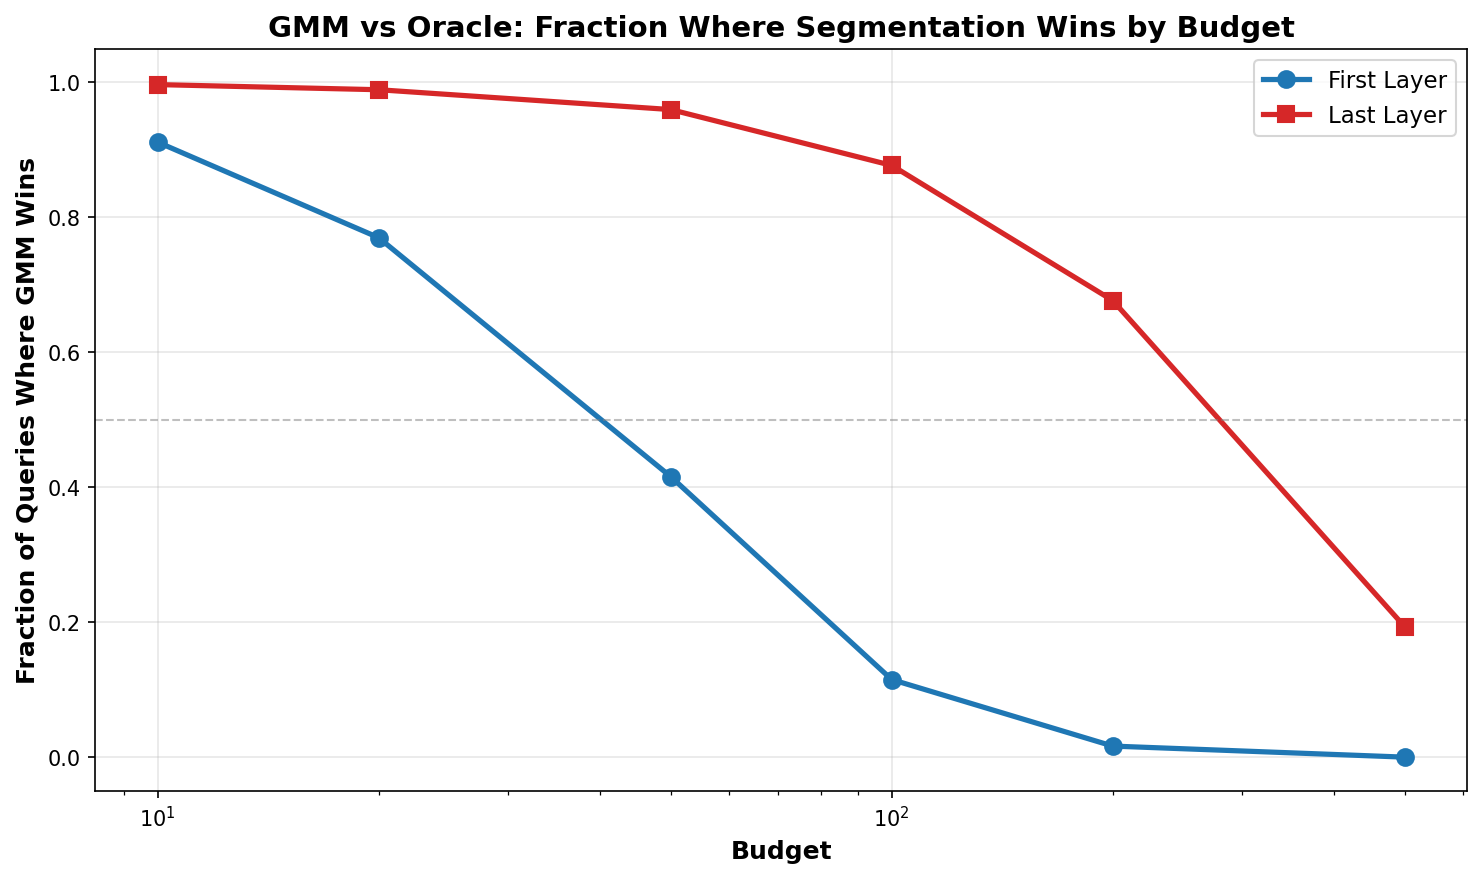
\includegraphics[width=0.85\textwidth]{figures/seg_wins_by_budget.png}
\caption{Fraction of queries where segmentation ($C{=}50$) beats oracle
  sampling, as a function of sampling budget~$B$.  At the last layer,
  segmentation wins for nearly all queries at low budgets ($B \le 50$) and
  retains an advantage up to $B \approx 300$.  At the first layer, the
  crossover occurs much earlier ($B_{\mathrm{cross}} \approx 42$).}
\label{fig:seg-wins}
\end{figure}

\begin{figure}[ht]
\centering
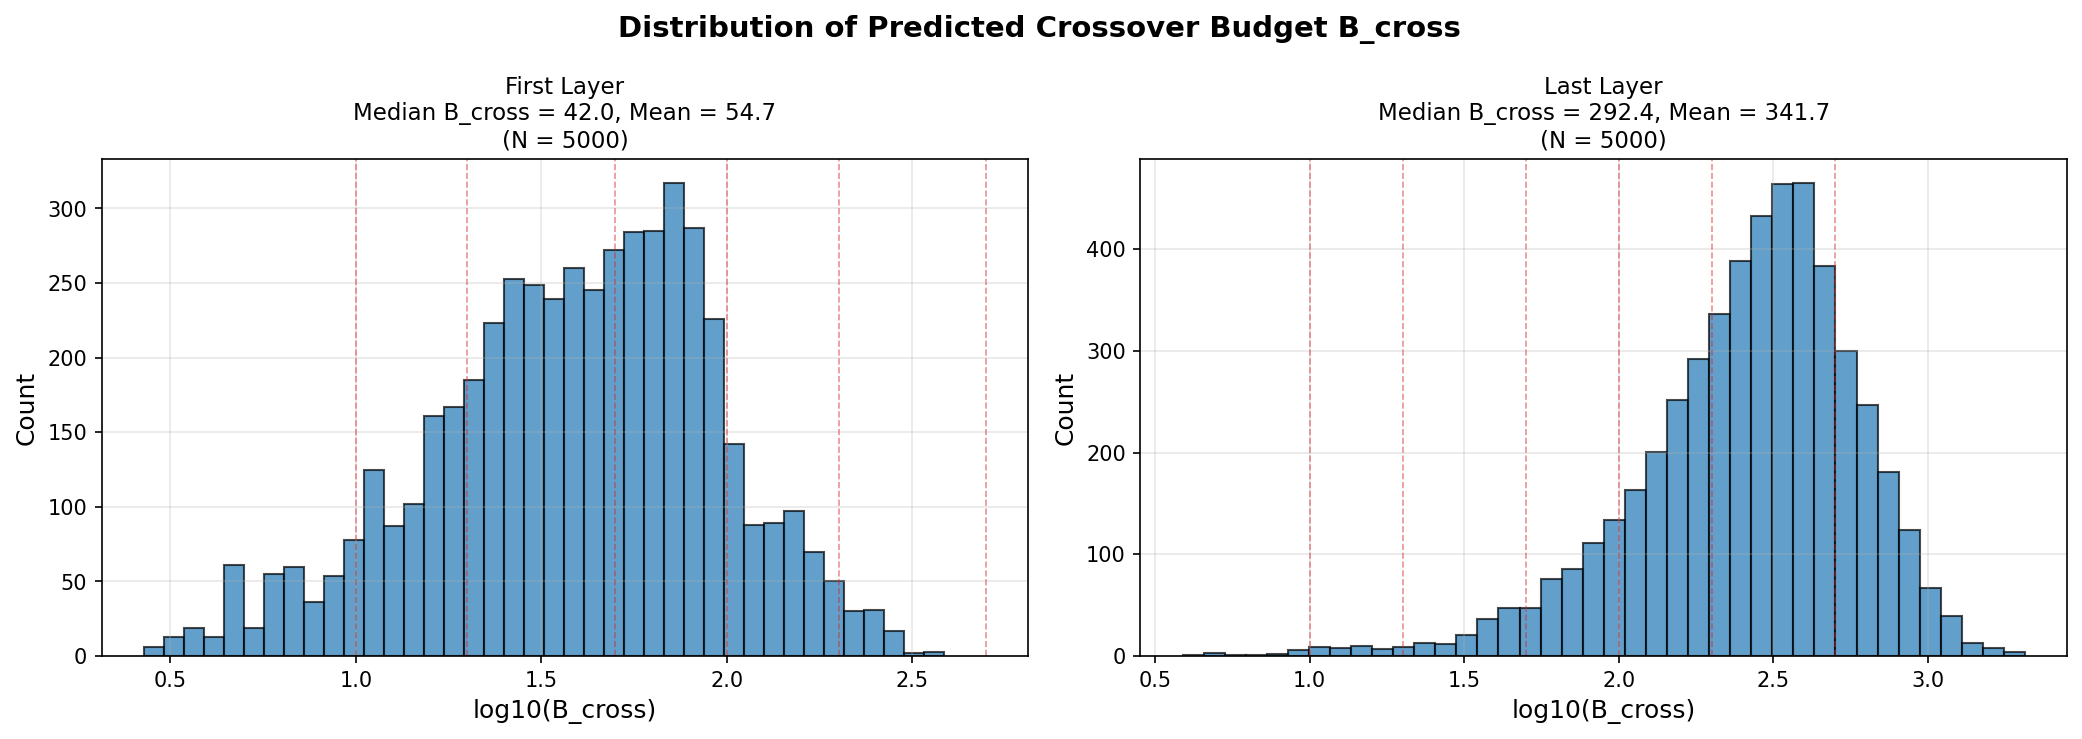
\includegraphics[width=0.85\textwidth]{figures/bcross_distribution.png}
\caption{Distribution of the crossover budget $B_{\mathrm{cross}}$ across
  queries.  The first layer (left) has a low median (${\sim}42$), while the
  last layer (right) has a much higher median (${\sim}292$), reflecting the
  $367\times$ difference in $\Var_w(\mathbf{V})$.}
\label{fig:bcross-dist}
\end{figure}

Table~\ref{tab:seg-wins} shows how the fraction of queries where segmentation
wins varies with budget.

\begin{table}[ht]
\centering
\small
\begin{tabular}{lcccccc}
\toprule
& $B{=}10$ & $B{=}25$ & $B{=}50$ & $B{=}100$ & $B{=}200$ & $B{=}500$\\
\midrule
First layer  & 91\% & 61\% & 35\% & 12\% & 2\% & 0\%\\
Last layer   & 100\% & 99\% & 97\% & 88\% & 65\% & 19\%\\
\bottomrule
\end{tabular}
\caption{Fraction of queries where GMM segmentation ($C{=}50$) achieves lower
error than oracle sampling at budget~$B$.}
\label{tab:seg-wins}
\end{table}

% ──────────────────────────────────────────────────────────────────
\subsection{Bias Source Ablation}\label{sec:exp-ablation}

To disentangle the two bias sources from Section~\ref{sec:two-sources}, we
compare four variants of GMM segmentation at $C=50$:
\begin{itemize}[nosep]
  \item \textbf{Standard}: approximate weights $\hat{w}_c$ and approximate
    values $\bar{\vv}_c$ (the default GMM estimator).
  \item \textbf{Exact Weights}: replace $\hat{w}_c$ with true cluster masses
    $W_c = \sum_{i \in S_c} w_i$, keep approximate values.
  \item \textbf{Exact Values}: keep approximate weights, replace $\bar{\vv}_c$
    with true attention-weighted means $\bmu_c$.
  \item \textbf{Exact Both}: use true $W_c$ and true $\bmu_c$ (tests partition
    quality alone).
\end{itemize}
Oracle sampling at $B{=}50$ is included as a sampling baseline.

\begin{center}
\small
\begin{tabular}{lccccc}
\toprule
& Standard & Exact Wt & Exact Val & Exact Both & Oracle\\
\midrule
First layer  & 0.555 & \textbf{0.091} & 0.536 & ${\sim}10^{-6}$ & 0.492\\
Last layer   & 0.149 & \textbf{0.080} & 0.122 & ${\sim}10^{-6}$ & 0.288\\
\bottomrule
\end{tabular}
\end{center}

\begin{figure}[ht]
\centering
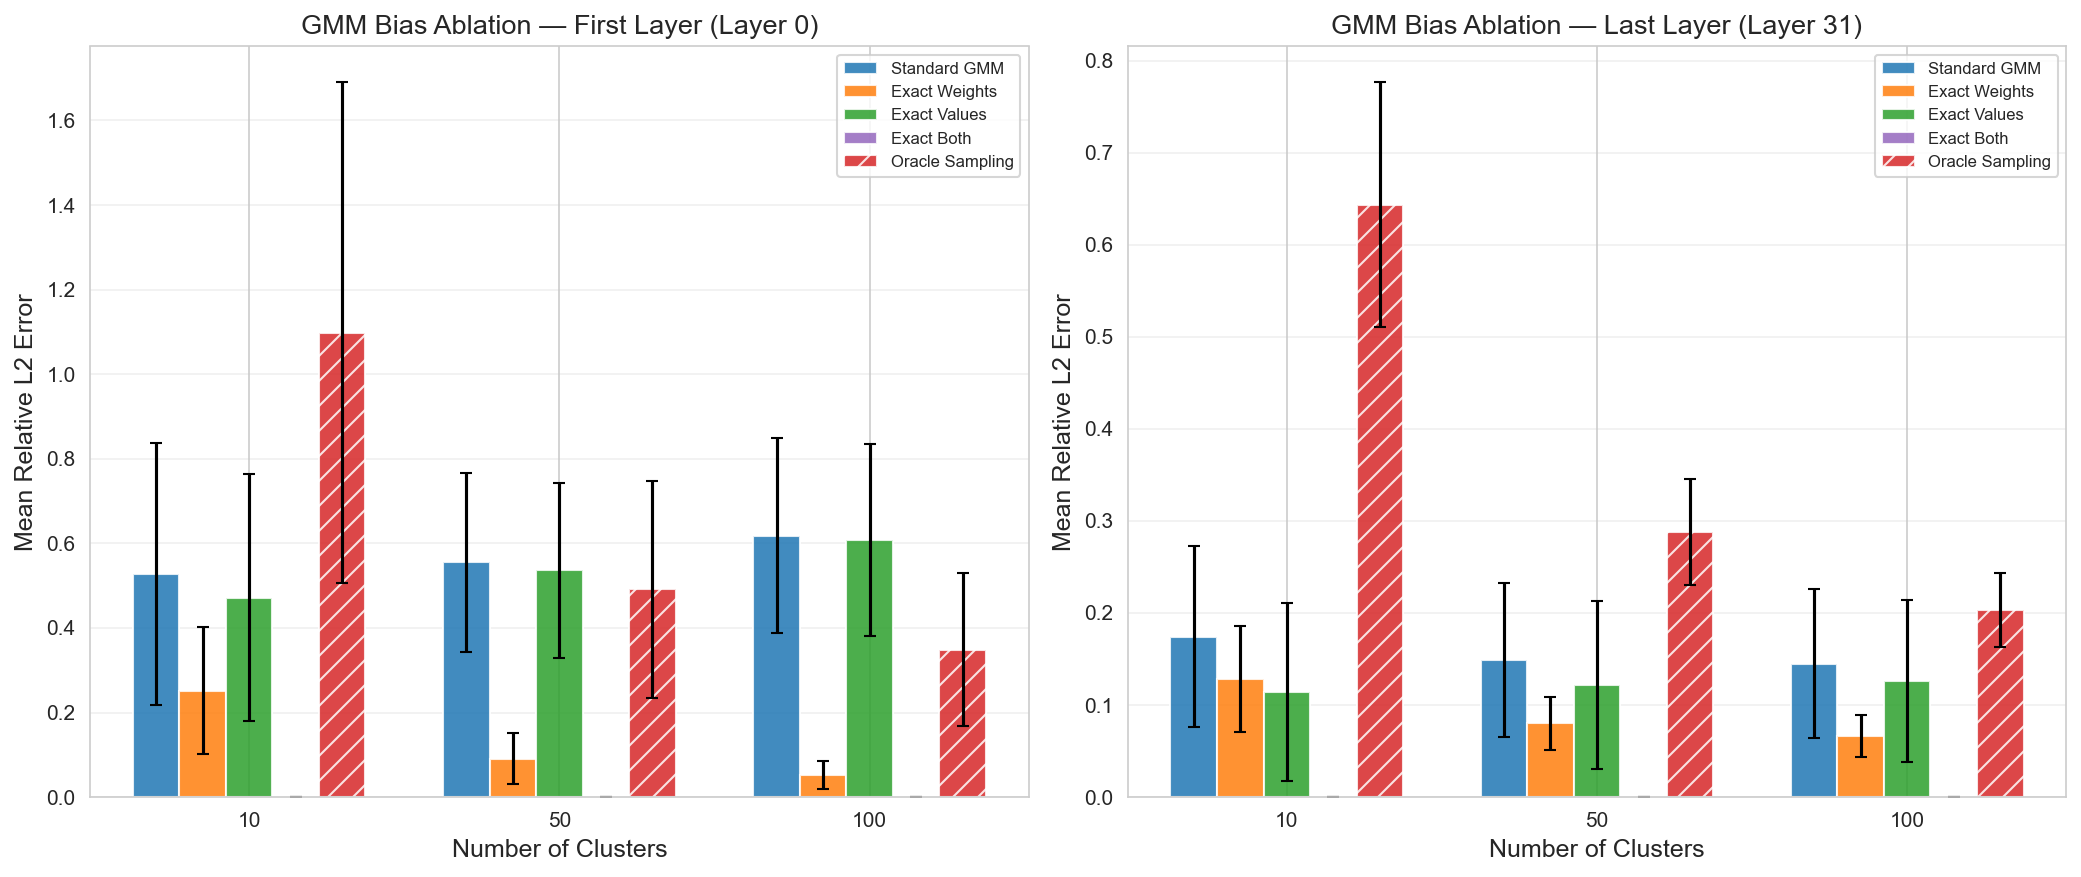
\includegraphics[width=0.85\textwidth]{figures/bias_ablation.png}
\caption{Ablation of bias sources in GMM segmentation ($C{=}50$).
  \emph{Exact Weights} (fixing weight distortion) reduces error by 84\% at
  the first layer and 46\% at the last layer.
  \emph{Exact Values} (fixing value averaging) yields only 3\% and 18\%
  reductions respectively.  \emph{Exact Both} confirms the partition is
  near-perfect (${\sim}10^{-6}$ error).}
\label{fig:ablation}
\end{figure}

\noindent\textbf{Key findings.}
\begin{enumerate}[nosep]
  \item \textbf{Weight distortion dominates}: fixing weights alone reduces
    error by 84\% (first layer) and 46\% (last layer).  Value averaging
    contributes only 3\% (first) and 18\% (last) of the total error.
  \item \textbf{Partition quality is near-perfect}: Exact Both achieves
    ${\sim}10^{-6}$ error, confirming that the GMM partition itself is
    excellent---the bias comes entirely from the centroid-softmax weight
    approximation and value averaging, not from poor cluster assignments.
  \item \textbf{With exact weights, GMM beats oracle}: at the first layer,
    Exact Weights (0.091) outperforms oracle sampling (0.492) by $5.4\times$,
    showing that segmentation's advantage can be dramatic when weight
    distortion is eliminated.
\end{enumerate}

% ──────────────────────────────────────────────────────────────────
\subsection{$K$-Means vs.\ GMM Partition}\label{sec:exp-kmeans}

To test whether the non-monotonicity from Section~\ref{sec:nonmono} is a
fundamental tradeoff or a GMM fitting artifact, we compare $k$-means and GMM
partitions across cluster counts.

\begin{center}
\small
\begin{tabular}{lcccccc}
\toprule
& $C{=}10$ & $C{=}20$ & $C{=}50$ & $C{=}100$ & $C{=}200$ & $C{=}500$\\
\midrule
\multicolumn{7}{l}{\emph{Last layer:}}\\
\quad GMM      & 0.171 & 0.157 & \textbf{0.147} & 0.156 & 0.172 & 0.195\\
\quad $K$-means & 0.177 & 0.158 & 0.149 & 0.141 & 0.138 &
  \textbf{0.118}\\
\midrule
\multicolumn{7}{l}{\emph{First layer:}}\\
\quad GMM      & 0.523 & 0.552 & 0.570 & 0.648 & 0.729 & 1.007\\
\quad $K$-means & 0.519 & 0.511 & 0.564 & 0.573 & 0.594 & 0.757\\
\bottomrule
\end{tabular}
\end{center}

\begin{figure}[ht]
\centering
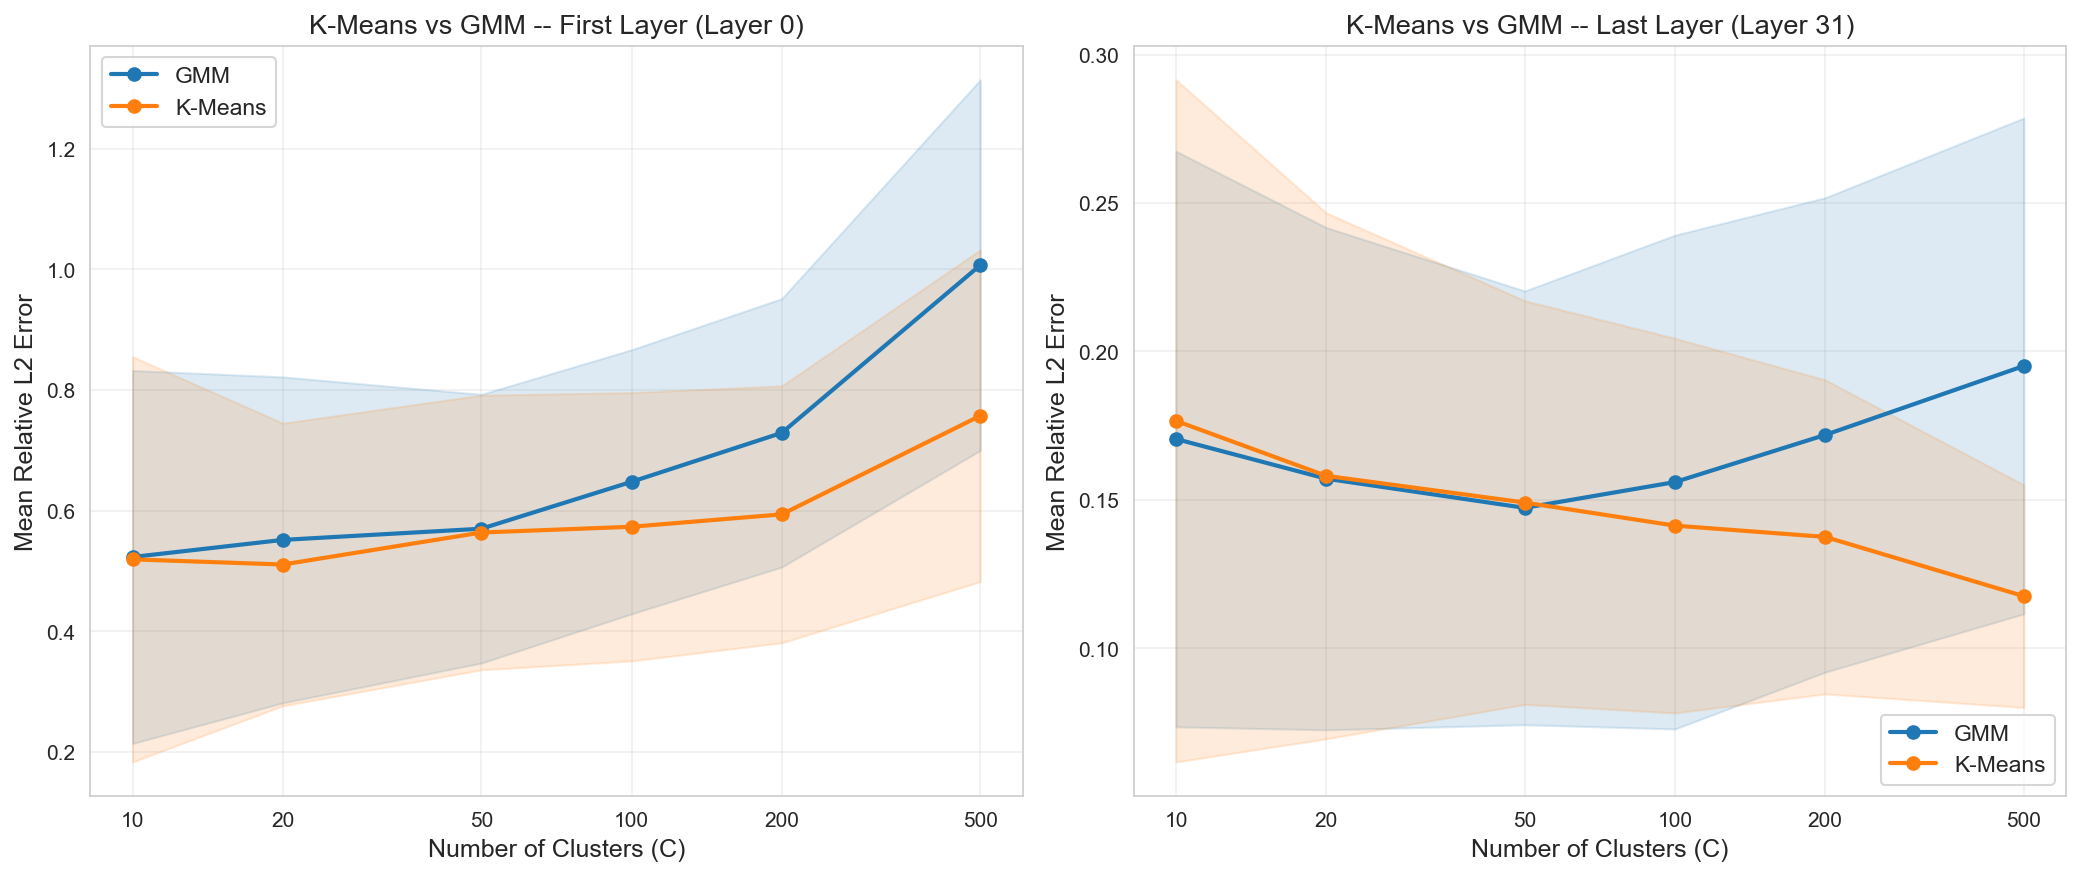
\includegraphics[width=0.85\textwidth]{figures/kmeans_vs_gmm.png}
\caption{GMM vs.\ $k$-means segmentation error across cluster counts.  At the
  last layer, $k$-means error decreases monotonically ($0.177 \to 0.118$),
  while GMM error U-shapes (best at $C{=}50$, degrades beyond).  GMM retains a
  slight edge at small~$C$ due to soft assignment regularization.}
\label{fig:kmeans-gmm}
\end{figure}

\noindent\textbf{Key findings.}
\begin{enumerate}[nosep]
  \item The non-monotonicity is \textbf{a GMM fitting artifact}: $k$-means
    error decreases monotonically with $C$ (last layer: $0.177 \to 0.118$).
  \item GMM retains a slight advantage at small $C$ ($\le 20$), likely because
    soft assignment acts as a regularizer on the value representatives.
  \item At large $C$ ($\ge 100$), $k$-means is substantially better: 10--40\%
    lower error, because hard assignment avoids the EM convergence issues that
    plague GMM with few points per component in $d{=}128$.
\end{enumerate}

% ──────────────────────────────────────────────────────────────────
\subsection{Nearest-Value Key Selection (Strategy~A$'$)}\label{sec:exp-nnkey}

We test Strategy~A$'$ (Section~\ref{sec:strat-nvk}), which replaces the
averaged centroid key $\bar{\kk}_c$ with the key of the element whose value is
closest to the value centroid.

\begin{center}
\small
\begin{tabular}{lccc}
\toprule
& $C{=}10$ & $C{=}50$ & $C{=}100$\\
\midrule
\multicolumn{4}{l}{\emph{Last layer:}}\\
\quad Strategy~A (standard)  & 0.169 & 0.140 & 0.135\\
\quad Strategy~A$'$ (NN key) & 0.258 & 0.182 & 0.158\\
\quad Degradation            & +53\% & +30\% & +17\%\\
\midrule
\multicolumn{4}{l}{\emph{First layer:}}\\
\quad Strategy~A (standard)  & 0.524 & 0.548 & 0.613\\
\quad Strategy~A$'$ (NN key) & 0.948 & 0.756 & 0.731\\
\quad Degradation            & +81\% & +38\% & +19\%\\
\bottomrule
\end{tabular}
\end{center}

\begin{figure}[ht]
\centering
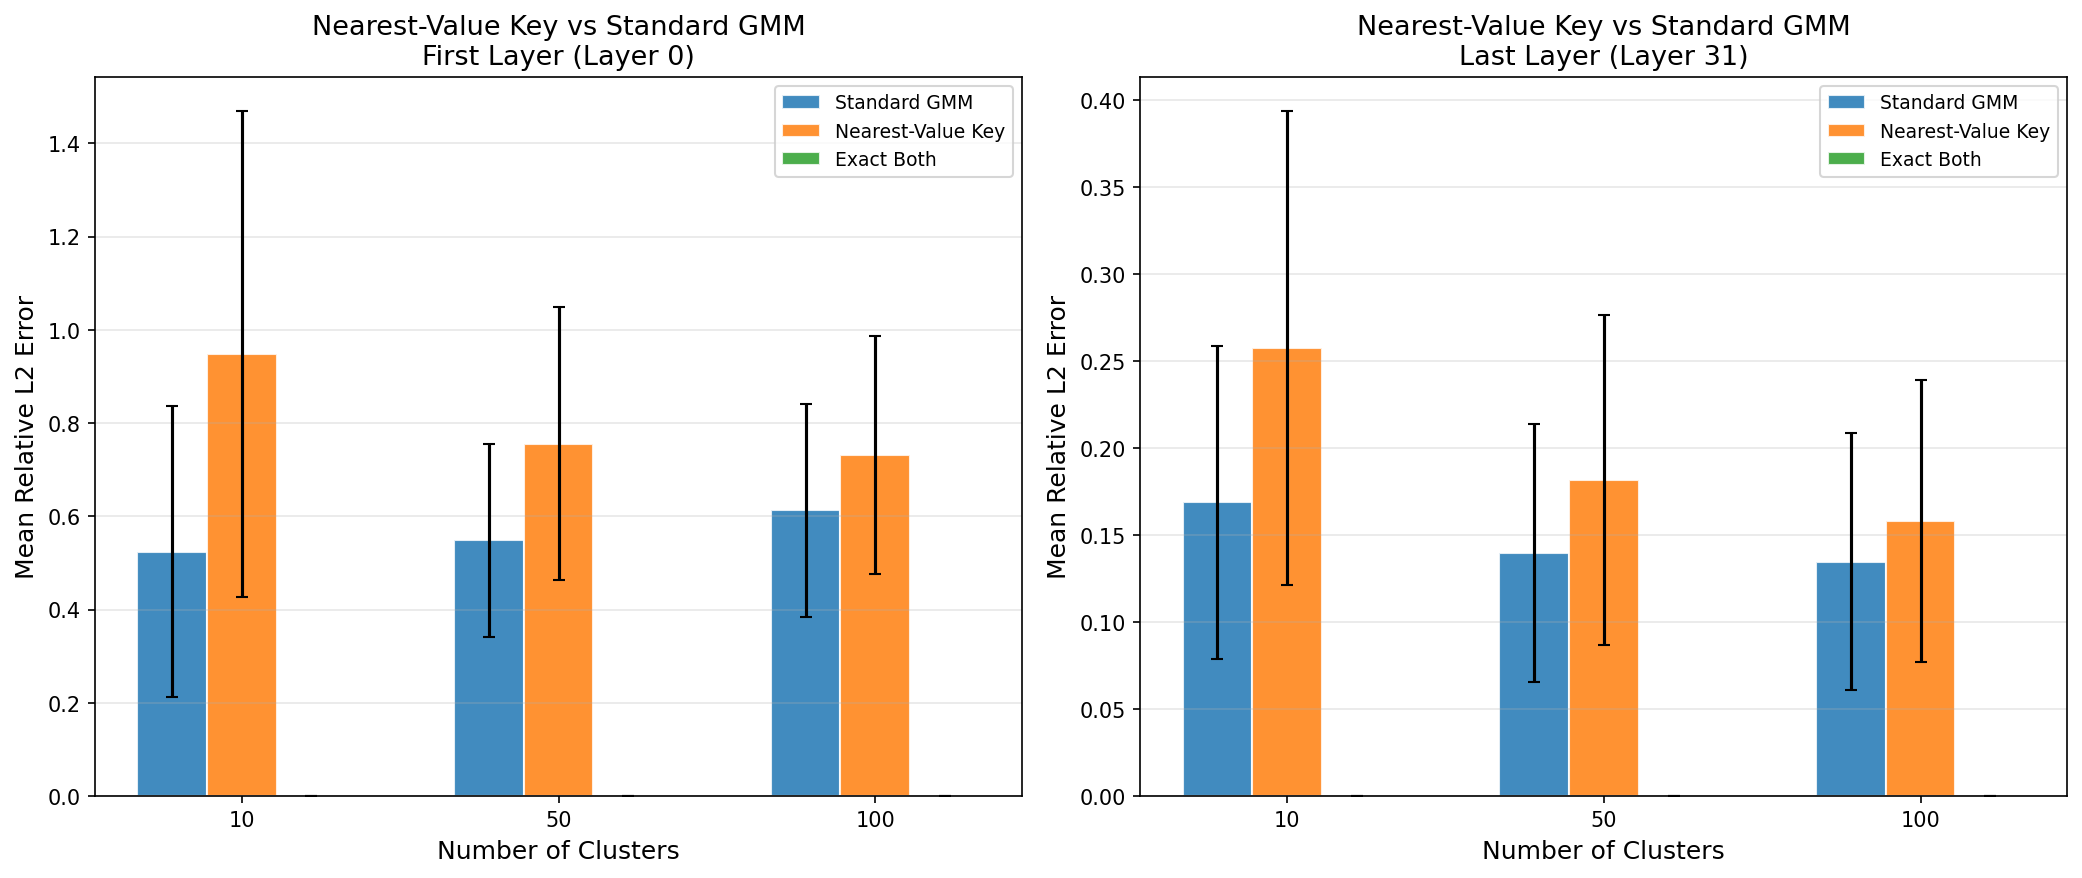
\includegraphics[width=0.85\textwidth]{figures/strategy_a_prime.png}
\caption{Strategy~A (averaged centroid key) vs.\ Strategy~A$'$ (nearest-value
  key selection).  A$'$ is uniformly worse across all cluster counts and
  both layers, with 17--81\% degradation.}
\label{fig:strategy-aprime}
\end{figure}

\noindent\textbf{Key findings.}
Strategy~A$'$ is \textbf{uniformly worse} than Strategy~A.  The selection bias
from using a single key to represent an entire cluster exceeds the Jensen
averaging bias of the centroid key.  This is a clean negative result for
item~2 of Conjecture~\ref{conj:strategy}: Strategy~A$'$ does not improve over
Strategy~A even when $\sigma_c^2$ is nontrivial (0.321 at the last layer).
The Exact Both baseline (${\sim}10^{-6}$) from the ablation confirms that the
partition itself is near-perfect, so the failure is specifically in the
weight computation.


% ══════════════════════════════════════════════════════════════════
\section{Analogies to Statistical Physics}\label{sec:physics}

The clustering approach admits suggestive (though informal) connections to
statistical physics.

\paragraph{Block spin renormalization.}
Replacing a group of key--value pairs with a single representative is
analogous to \emph{block spin renormalization} (Kadanoff, 1966): a block of
spins is replaced by a single effective spin, with renormalized coupling
constants derived from the original ones.  In our setting, the centroid logit
$\bar{z}_c$ plays the role of the renormalized coupling.  The approximation
is exact when within-block fluctuations vanish (within-cluster value
homogeneity).

\paragraph{Gibbs distribution viewpoint.}
The attention weights $w_i$ form a Gibbs distribution
$p(i) = e^{z_i}/Z$ with energy $E_i = -z_i$.  The segmentation produces a
coarse-grained Gibbs distribution over $C$ states.  The KL divergence between
fine and coarse distributions,
$\KL(p\|p_{\mathrm{coarse}}) = \sum_c W_c H_c$
(where $H_c$ is the within-cluster relative entropy), quantifies the
information lost in coarse-graining.

\begin{researchnote}
These analogies are informal.  In mean field theory, there are genuine
spin--spin interactions that are approximated by an average field.  In
standard attention, the query--key interactions are independent; the coupling
arises only through the softmax normalization.  The structural parallel is
suggestive but not precise.  The KL formula is correct algebra, but the GMM
does not minimize this KL---it minimizes the key-space likelihood, a
different objective.  These connections should be taken as motivation, not as
formal results.
\end{researchnote}


% ══════════════════════════════════════════════════════════════════
\section{Towards Optimal Algorithm Selection}\label{sec:selection}

Given query $\qq$, keys $\mathbf{K}$, values $\mathbf{V}$, and budget $B$,
the theoretically optimal strategy depends on:

\begin{enumerate}[nosep]
  \item \textbf{Attention concentration}: if entropy
    $H(w) < \log B$, TopK suffices.
  \item \textbf{Clustering quality}: the ratio
    $\rho = \sum_c W_c\|\bmu_c-\oo^*\|^2 / \Var_w(\mathbf{V})$
    (proportion of variance captured by the partition).
  \item \textbf{Budget level}: low $B$ favors segmentation; high $B$ favors
    sampling.
\end{enumerate}

\begin{researchnote}
This decision framework is theoretically clean but \emph{not directly
applicable} at inference time: computing $H(w)$, $\rho$, or $\Var_w(\mathbf{V})$
requires the exact attention weights (the full $O(N)$ computation).  A
practical algorithm selection rule would need cheap proxies---for instance,
estimating attention concentration from key norm statistics or a small
subsample of logits.  Developing such proxies is an important open problem.
\end{researchnote}


% ══════════════════════════════════════════════════════════════════
\section{Summary of Theoretical Results}\label{sec:summary}

\begin{theorem}[Sampling variance lower bound]
For any IS proposal $q$,
\[
  \Tr(\Cov(\hat{\oo}_{\mathrm{IS}}))
  \;\ge\;
  \frac{1}{B}\Bigl[
    \Bigl(\sum_i w_i\|\vv_i\|\Bigr)^{2} - \|\oo^{*}\|^{2}
  \Bigr],
\]
with equality at $q_i^*\propto w_i\|\vv_i\|$.
\end{theorem}

\begin{theorem}[Variance decomposition (Cochran--Rao-Blackwell)]
\[
  \Var_w(\mathbf{V})
  = \sum_c W_c\Var_{w|c}(\mathbf{V})
  + \sum_c W_c\|\bmu_c - \oo^{*}\|^{2}.
\]
Stratified sampling eliminates the between-cluster term.
\end{theorem}

\begin{proposition}[Softmax sensitivity]
$\|\Delta\ww\|_2 \le \max_i w_i\cdot\|\Delta\zz\|_2$.
\end{proposition}

\begin{conjecture}[Segmentation bias bound]\label{conj:bias}
For a partition with within-cluster logit range $\Delta_c$ and within-cluster
value diameter $\epsilon_c$, the GMM-style segmentation error satisfies
\[
  \|\hat{\oo}_{\mathrm{seg}} - \oo^{*}\|
  \;\lesssim\;
  \underbrace{f(\{\Delta_c\},\{\hat{w}_c\})\cdot\max_i\|\vv_i\|}
    _{\text{weight distortion}}
  \;+\; \underbrace{\max_c\epsilon_c}_{\text{value averaging}}
  \;+\; \underbrace{\text{cross-term}}_{\text{to be bounded}},
\]
where $f$ captures the propagation of per-cluster Jensen gaps through the
softmax normalization.
\end{conjecture}

\begin{researchnote}
Conjecture~\ref{conj:bias} is the main open theoretical problem.  Making this
rigorous requires bounding the function $f$---specifically, how the
multiplicative underestimation factors $(1+\sigma_c^2/2)$ per cluster
interact through the softmax denominator.  The cross-term from the
decomposition~\eqref{eq:three-term} must also be controlled.  A clean bound
here would be a significant contribution.
\end{researchnote}


% ══════════════════════════════════════════════════════════════════
\section{Open Problems and Required Experiments}\label{sec:open}

\subsection{Theoretical}
\begin{enumerate}[nosep]
  \item Rigorous end-to-end MSE bound for segmentation with centroid-softmax
    weights (proving Conjecture~\ref{conj:bias}).
  \item Rigorous comparison of RFF-based vs.\ centroid-softmax weights,
    accounting for softmax normalization.
  \item Optimal partition criterion: should we cluster in key space, value
    space, or a weighted combination?
  \item Connection to James-Stein shrinkage: in $d=128$ dimensions, can the
    segmentation bias be understood as beneficial shrinkage?
\end{enumerate}

\subsection{Empirical (Completed)}
The following have been resolved by the experiments in
Section~\ref{sec:experiments}:
\begin{enumerate}[nosep]
  \item[\checkmark] \textbf{Per-layer diagnostics}
    (Section~\ref{sec:exp-diagnostics}): all four intuitive hypotheses
    contradicted; $\Var_w(\mathbf{V})$ identified as the dominant driver.
  \item[\checkmark] \textbf{Bias source ablation}
    (Section~\ref{sec:exp-ablation}): weight distortion dominates (84\%/46\%
    of error at first/last layer).
  \item[\checkmark] \textbf{GMM convergence at large $C$}
    (Section~\ref{sec:exp-kmeans}): non-monotonicity is a GMM fitting
    artifact; $k$-means is monotone.
  \item[\checkmark] \textbf{Crossover budget measurement}
    (Section~\ref{sec:exp-crossover}): formula validated with log-correlation
    0.96, 89\% within $2\times$.
\end{enumerate}

\subsection{Empirical (Open)}
\begin{enumerate}[nosep]
  \item \textbf{PCA on key vectors}: measure effective dimensionality
    $d_{\mathrm{eff}}$ to test the low-intrinsic-dimensionality hypothesis
    from Section~\ref{sec:dimension}.
  \item \textbf{Full strategy comparison}: implement Strategies~B--D from
    Section~\ref{sec:disentangle} (RFF weights, within-cluster IS, hybrid).
    Strategy~A$'$ has been tested and rejected
    (Section~\ref{sec:exp-nnkey}).
  \item \textbf{Weight correction method}: the ablation
    (Section~\ref{sec:exp-ablation}) shows the Jensen correction
    $\sigma_c^2/2$ could yield large gains.  Design a practical estimator
    for $\sigma_c^2$ that does not require evaluating all $N$ logits.
  \item \textbf{$K$-means at very large $C$}: extend the comparison from
    Section~\ref{sec:exp-kmeans} to $C > 500$ to determine the asymptotic
    behavior as $C \to N$.
  \item \textbf{Layer-adaptive selection policy}: given the $367\times$
    difference in $\Var_w(\mathbf{V})$, design a per-layer rule that selects
    sampling for early layers and segmentation for later layers.
\end{enumerate}


% ══════════════════════════════════════════════════════════════════
\bibliographystyle{plain}

\begin{thebibliography}{99}

\bibitem{cochran1977}
W.~G. Cochran.
\newblock {\em Sampling Techniques}.
\newblock Wiley, 3rd edition, 1977.

\bibitem{owen2013}
A.~B. Owen.
\newblock {\em Monte Carlo Theory, Methods and Examples}.
\newblock 2013.

\bibitem{robert2004}
C.~P. Robert and G.~Casella.
\newblock {\em Monte Carlo Statistical Methods}.
\newblock Springer, 2nd edition, 2004.

\bibitem{gersho1992}
A.~Gersho and R.~M. Gray.
\newblock {\em Vector Quantization and Signal Compression}.
\newblock Springer, 1992.

\bibitem{wainwright2008}
M.~J. Wainwright and M.~I. Jordan.
\newblock Graphical models, exponential families, and variational inference.
\newblock {\em Foundations and Trends in Machine Learning}, 1(1--2):1--305,
  2008.

\bibitem{chen2024magicpig}
T.~Chen et~al.
\newblock {MagicPIG}: {LSH} sampling for efficient {LLM} generation.
\newblock {\em arXiv:2410.16179}, 2024.

\bibitem{vyas2020clustered}
A.~Vyas, A.~Katharopoulos, and F.~Fleuret.
\newblock Fast transformers with clustered attention.
\newblock In {\em NeurIPS}, 2020.

\bibitem{kitaev2020reformer}
N.~Kitaev, {\L}.~Kaiser, and A.~Levskaya.
\newblock Reformer: The efficient transformer.
\newblock In {\em ICLR}, 2020.

\bibitem{choromanski2021rethinking}
K.~Choromanski et~al.
\newblock Rethinking attention with performers.
\newblock In {\em ICLR}, 2021.

\bibitem{wang2020linformer}
S.~Wang et~al.
\newblock Linformer: Self-attention with linear complexity.
\newblock {\em arXiv:2006.04768}, 2020.

\bibitem{xiong2022nystromformer}
Y.~Xiong et~al.
\newblock Nystr\"{o}mformer: A {Nystr\"{o}m}-based algorithm for
  approximating self-attention.
\newblock In {\em AAAI}, 2022.

\bibitem{kadanoff1966}
L.~P. Kadanoff.
\newblock Scaling laws for {Ising} models near ${T}_c$.
\newblock {\em Physics}, 2(6):263--272, 1966.

\bibitem{caflisch1998}
R.~E. Caflisch.
\newblock Monte {C}arlo and quasi-{M}onte {C}arlo methods.
\newblock {\em Acta Numerica}, 7:1--49, 1998.

\bibitem{rahimi2007random}
A.~Rahimi and B.~Recht.
\newblock Random features for large-scale kernel machines.
\newblock In {\em NeurIPS}, 2007.

\end{thebibliography}

\end{document}
